% =====================================================================
%  PRL letter
%  Compile: pdflatex main ; pdflatex main   (references are inline)
%  Figures: figures/fig2_srs.pdf, figures/fig3_hierarchy.pdf,
%           figures/fig4_maps_creep.pdf
%  Items marked \todo{} must be completed before submission.
% =====================================================================
\documentclass[aps,prl,twocolumn,superscriptaddress,amsmath,amssymb,floatfix]{revtex4-2}

\usepackage{graphicx}
\usepackage{bm}
\usepackage{xcolor}
\usepackage{tikz}
\usetikzlibrary{arrows.meta,positioning,fit,calc}
\usepackage[colorlinks=true,citecolor=blue!50!black,linkcolor=blue!50!black,urlcolor=blue!50!black]{hyperref}

\newcommand{\gd}{\dot\gamma}
\newcommand{\ts}{\tau^{\star}}
\newcommand{\kT}{k_BT}
\newcommand{\todo}[1]{\textcolor{red}{[#1]}}
\newcommand{\fig}[2]{\IfFileExists{figures/#1}{\includegraphics[width=#2]{figures/#1}}{\fbox{\parbox[c][3cm][c]{#2}{\centering figures/#1}}}}

\begin{document}

\title{Unified kinetic description of flow stress, strain-rate sensitivity, dynamic strain aging, and creep in body-centered-cubic metals}

\author{Matthew Maron}
\affiliation{\todo{Affiliation}}
\author{Giacomo Po}
\affiliation{\todo{Affiliation}}
\author{Yang Li}
\affiliation{\todo{Affiliation}}

\date{\today}

\begin{abstract}
The strain-rate sensitivity of body-centered-cubic metals varies non-monotonically with temperature, becomes negative under dynamic strain aging, and grows sharply as plastic flow turns into creep. We show that all of these regimes follow from one kinetic flow rule. Kink-pair glide sets the mobility, and a microstructural state, comprising forest density, solute atmospheres and particle pinning, sets the resistance; the state evolves under kinetics fixed by the imposed rate and temperature but not by the stress. The flow stress is therefore single valued everywhere, including where it decreases with rate, and no switching functions are required. Differentiating the rule gives an exact decomposition of the rate sensitivity, $1/m=\tau A/(1+\Lambda)$, in which $A$ measures the mobility and $\Lambda$ the rate dependence of the resistance; negative $m$ corresponds exactly to $\Lambda<-1$. A nested hierarchy of the same rule, built up from W to Zr to the ferritic-martensitic steel Eurofer-97, reproduces flow stresses, rate sensitivities and activation volumes from room temperature to 1000~K, and the minimum creep rates of Eurofer-97 over five decades.
\end{abstract}

\maketitle

% ---------------------------------------------------------------------
Plastic flow of body-centered-cubic (BCC) metals, and of prismatic slip in hexagonal Zr and Ti, is controlled at low temperature by the thermally activated nucleation of kink pairs on screw dislocations~\cite{HirthLothe,Po2016}. With increasing temperature the flow stress falls onto an athermal plateau, often develops a hump associated with dynamic strain aging (DSA)~\cite{Cheng2001,KubinEstrin1990}, and finally drops steeply as diffusion-controlled recovery and climb set in~\cite{FrostAshby}. The strain-rate sensitivity $m=\partial\ln\tau/\partial\ln\gd$ and the apparent activation volume $V^\star=\kT/(m\tau)$ are the standard probes of this sequence, and their temperature dependence is routinely read as a succession of rate-controlling mechanisms.

That reading is ambiguous. The same non-monotonic $m(T)$ can arise from a single mechanism whose athermal share of the stress changes, from solute aging, or from recovery. Constitutive descriptions reflect the ambiguity: stresses from different mechanisms are added~\cite{Seeger,KocksArgonAshby,EstrinMcCormick}, or strain rates are added~\cite{FrostAshby}, and the passage from one regime to the next is imposed through onset functions of temperature. What is missing is a single rule from which the regimes, their boundaries and the measured $m$ and $V^\star$ all follow, together with a way to tell from experiment which part of the physics controls the rate sensitivity.

Here we construct such a rule and show that it can be built up hierarchically. Its minimal form, kink-pair mobility acting against a forest, describes W. Adding solute aging and diffusion-controlled recovery of the same forest describes Zr, including its negative rate sensitivity. Adding boundary storage and particle pinning with thermal and climb bypass describes Eurofer-97 in tension and in creep. Each level contains the previous one unchanged (Fig.~\ref{fig:scheme}).

% ---------------------------------------------------------------------
\begin{figure}[b]
\centering
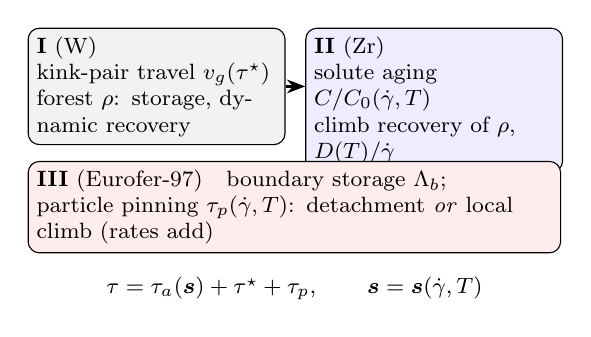
\begin{tikzpicture}[font=\footnotesize,>=Stealth,
  lvl/.style={draw,rounded corners,align=left,inner sep=3pt}]
  \node[lvl,fill=gray!10,text width=3.05cm] (I) {\textbf{I} (W)\\ kink-pair travel $v_g(\ts)$\\ forest $\rho$: storage, dynamic recovery};
  \node[lvl,fill=blue!7,text width=3.05cm,right=0.25cm of I.north east,anchor=north west] (II) {\textbf{II} (Zr)\\ solute aging $C/C_0(\gd,T)$\\ climb recovery of $\rho$, $D(T)/\gd$};
  \node[lvl,fill=red!7,text width=6.55cm,below=0.2cm of I.south west,anchor=north west] (III) {\textbf{III} (Eurofer-97)\quad boundary storage $\Lambda_b$;\\ particle pinning $\tau_p(\gd,T)$: detachment \emph{or} local climb (rates add)};
  \node[align=center,below=0.18cm of III] {$\tau=\tau_a(\bm s)+\ts+\tau_p,\qquad \bm s=\bm s(\gd,T)$};
  \draw[->,thick] (I.east) -- (II.west |- I.east);
\end{tikzpicture}
\caption{Nested hierarchy of the flow rule. Each level adds microstructural physics to the one before it and leaves the lower level unchanged. The state $\bm s$ depends on the imposed rate and temperature but not on the stress.}
\label{fig:scheme}
\end{figure}

% ---------------------------------------------------------------------
Plastic shear is carried by mobile dislocations of density $\rho_m$ and Burgers vector $b$ moving at a mean velocity $\bar v$~\cite{Orowan1940},
\begin{equation}
\gd=\rho_m\,b\,\bar v .
\label{eq:orowan}
\end{equation}
The model is contained entirely in how $\bar v$ is written. A segment does not move steadily: over one characteristic glide distance $\lambda$ it spends a time $t_r$ travelling through the lattice and a time $t_w$ waiting at obstacles it cannot pass immediately, so that $\bar v=\lambda/(t_r+t_w)$ and
\begin{equation}
\frac{1}{\gd}=\frac{t_r+t_w}{\rho_mb\lambda}.
\label{eq:inv_rate}
\end{equation}
Between obstacles the segment glides at the lattice velocity $v_g(\ts)$, where $\ts$ is the effective stress on the lattice-friction process; with $t_r=\lambda/v_g$ the travel term is $1/\rho_mb\,v_g$, the rate the material would have if travel were the only process. If obstacle populations $j$ have areal densities $\lambda_j^{-2}$ on the slip plane, a segment meets $n_j=\lambda_j^{-2}\lambda$ of them per unit glide distance, with $\lambda^{-2}=\sum_j\lambda_j^{-2}$ the combined spacing, and waits $1/\nu_j$ at each, so the waiting term is $\sum_jn_j/\rho_mb\nu_j$. An obstacle may be passed in more than one way, by thermally activated cutting or detachment, by climb, or by cross slip; these routes are alternatives, and whichever succeeds first releases the segment, so $\nu_j=\sum_k\nu_{jk}(\ts)$. Equation~(\ref{eq:inv_rate}) then reads
\begin{equation}
\frac{1}{\gd}=\frac{1}{\rho_mb\,v_g(\ts)}+\frac{1}{\rho_mb}\sum_j\frac{n_j}{\sum_k\nu_{jk}(\ts)} .
\label{eq:general}
\end{equation}
Processes met in sequence therefore add their times, so that the slowest step controls while every step contributes, and alternative routes past one obstacle add their rates, so that the fastest route controls.

Resistances that act on the line at the same time add their stresses instead. This applies to the long-range internal stresses, the Taylor forest stress and the boundary stresses, and to sparse strong obstacles that pin a line which is simultaneously held back by lattice friction, as in Kocks' superposition of dense-weak and sparse-strong populations~\cite{Seeger,KocksArgonAshby}:
\begin{equation}
\tau=\tau_a(\bm s)+\ts+\sum_g\tau_g(\gd,T),
\label{eq:flow}
\end{equation}
where $\tau_a$ is fixed by the microstructural state $\bm s$ and each superposed group $g$ obeys its own balance of the form of Eq.~(\ref{eq:general}). Which rule applies follows from the obstacle strength and spacing. Forest junctions in body-centered-cubic metals are strong and long ranged and enter $\tau_a$, their rate dependence coming through the forest density rather than through a waiting time; carbides and carbonitrides are sparse and much stronger than the lattice friction, so their stress superposes while their own time balance fixes it; weak, dense, thermally penetrable obstacles such as small clusters or irradiation loops would enter the waiting sum of Eq.~(\ref{eq:general}). None of the three metals treated here needs such a population, so the lattice term alone carries the imposed rate, $\gd=\rho_mb\,v_g(\ts)$.

The lattice velocity is the kink-pair law of Ref.~\cite{Po2016}, which combines the $(p,q)$ barrier profile of Kocks, Argon and Ashby~\cite{KocksArgonAshby} with kink-pair nucleation on long screw segments~\cite{DornRajnak1964,HirthLothe},
\begin{equation}
v_g=\frac{\ts b}{B_d}\exp\!\left\{-\frac{\Delta H_0}{2\kT}\left[\left(1-\left(\frac{\ts}{\tau_P}\right)^{p}\right)^{q}-\frac{T}{T_0}\right]\right\},
\label{eq:vg}
\end{equation}
in which $\ts b/B_d$ is the drag velocity with kink drag coefficient $B_d$, the activation enthalpy $\Delta H_0[1-(\ts/\tau_P)^p]^q$ vanishes at the Peierls stress $\tau_P$, the factor $1/2$ applies to long segments, where the rate is set by the square root of the nucleation rate times the kink migration rate, and $T/T_0$ acts as an entropic correction that removes the barrier above the athermal transition temperature.

The athermal stress is of Taylor form~\cite{Taylor1934,KocksMecking2003},
\begin{equation}
\tau_a=\alpha\,\mu(T)\,b\,\sqrt{C/C_0}\,\left(\sqrt{\rho_f}+\Lambda_b\right),
\label{eq:taua}
\end{equation}
where $\rho_f=\beta\rho$ is the forest part of the total density $\rho$ (with $\rho_m=f_m\rho_f$), $\Lambda_b$ is the inverse spacing of boundaries and $C/C_0$ is the solute enrichment defined below. The density follows Kocks--Mecking kinetics~\cite{Kocks1976,MeckingKocks,KocksMecking2003} extended by climb-controlled recovery,
\begin{equation}
\frac{d\rho}{d\gamma}=k_1\big(\sqrt\rho+\Lambda_b\big)-k_2\rho-\frac{K\,D(T)}{\gd}\,\rho^2 ,
\label{eq:km}
\end{equation}
in which $k_1\sqrt\rho$ is athermal storage at forest obstacles, $k_1\Lambda_b$ is storage at boundaries~\cite{EstrinMecking1984,Estrin1996} and $k_2\rho$ is dynamic recovery by cross slip and glide annihilation, which acts per unit strain. The last term is the classical second-order annihilation of dipoles and networks by climb, $d\rho/dt=-KD\rho^2$~\cite{SandstromLagneborg1975,Sandstrom1977,Nes1995,SandstromHallgren2012}, converted to a strain basis by dividing by $\gd$; unlike $k_2\rho$ it proceeds whether or not the crystal deforms, and its weight grows as $D/\gd$ increases. At steady state $\rho$ is the unique positive root of the right-hand side, and where the climb term dominates it gives $\tau_a\propto(\gd/D)^{1/3}$, the natural creep law of dislocation networks~\cite{Poirier1985,Blum2002}. Segments arrested at forest junctions of spacing $\lambda_f=\rho_f^{-1/2}$ wait for a time $t_a=\rho_mb\lambda_f/\gd$~\cite{McCormick1988,KubinEstrin1990}, during which solutes collect on them with Cottrell--Bilby kinetics~\cite{CottrellBilby} that saturate as described by Louat~\cite{Louat1981},
\begin{equation}
\frac{C}{C_0}=1+\sum_iC_i\left\{1-\exp\!\left[-\left(t_a\nu_ie^{-Q_i/\kT}\right)^{\alpha_i}\right]\right\},
\label{eq:aging}
\end{equation}
strengthening the junctions by $\sqrt{C/C_0}$~\cite{Cheng2001,MulfordKocks1979}.

A segment held at a particle escapes either by thermally activated detachment,
\begin{equation}
\nu_{\rm th}=\nu_0\exp\!\left\{-\frac{F}{\kT}\left[1-\left(\frac{\tau_p}{\hat\tau}\right)^{p}\right]^{q}\right\},
\label{eq:nuth}
\end{equation}
which reaches the Orowan limit as $\tau_p\to\hat\tau$~\cite{KocksArgonAshby,RoslerArzt}, or by climbing over it,
\begin{equation}
\nu_{\rm cl}=\frac{v_c}{h_{\rm eff}},\qquad
v_c=\frac{2\pi D}{b\ln(R/r_c)}\left[\exp\!\left(\frac{\tau_p\Omega}{\kT}\right)-1\right],
\label{eq:nucl}
\end{equation}
with the climb velocity of Ref.~\cite{HirthLothe} and a residual height $h_{\rm eff}=h(1-\tau_p/\hat\tau)$ that shrinks as the line is pressed against the particle, as in local-climb models~\cite{BrownHam,ArztAshby1982}. The two routes are alternatives, so their rates add and the particle stress follows from
\begin{equation}
\gd=\rho_mb\,\lambda_p\left[\nu_{\rm th}(\tau_p)+\nu_{\rm cl}(\tau_p)\right],
\label{eq:taup}
\end{equation}
with $\lambda_p$ the particle spacing. Because $\nu_{\rm cl}$ diverges as $\tau_p\to\hat\tau$, this route produces threshold-type creep with a stress exponent $(1-\tau_p/\hat\tau)^{-1}$ that falls as $D(T)$ grows. Diffusional flow~\cite{Nabarro1948,Herring1950,Coble1963,FrostAshby} transports matter rather than dislocations, so it is an independent carrier whose rate adds to that of the dislocation processes; it is negligible for the tensile and creep data treated here and is retained only for the deformation-mechanism maps.

The central structural property of this rule is that every state variable, $\rho$, $C/C_0$ and $\rho_m$, is fixed by $(\gd,T)$ and not by $\tau$. For a prescribed rate, $v_g$ is strictly increasing in $\ts$ and each $\nu$ is non-decreasing in $\tau_p$, so Eq.~(\ref{eq:flow}) has exactly one solution. The stress remains single valued even where aging makes it decrease with rate. Regime changes are not imposed; they emerge from the ratios $KD/\gd$, $t_a\nu e^{-Q/\kT}$ and $\nu_{\rm cl}/\nu_{\rm th}$, which are set by activation energies, diffusivities and spacings.

% ---------------------------------------------------------------------
This structure yields an exact decomposition of the rate sensitivity. Writing the intrinsic mobility as $\gd=G(\ts;\bm s)$ and differentiating Eq.~(\ref{eq:flow}) along the solution gives
\begin{equation}
\frac1m=\frac{\tau A}{1+\Lambda},\qquad
\Lambda\equiv AB,
\label{eq:srs}
\end{equation}
with
\begin{equation}
A=\frac{\partial\ln G}{\partial\ts},\qquad
B=\frac{d\tau}{d\ln\gd}-\frac1A .
\end{equation}
The mobility sensitivity $A$ is a property of the kink-pair barrier; $B$ collects the rate dependence of every resistance, through $\bm s(\gd,T)$ and $\tau_g(\gd,T)$. The activation volume becomes $V^\star=\kT A/(1+\Lambda)$. When $|\Lambda|\ll1$ the measured $V^\star$ is the mobility volume $\kT A$ and increases as the barrier softens. When $\Lambda\gg1$ it is $\kT/B$ and decreases as the resistance becomes more rate dependent. Aging strengthens the forest more at low rates, because slower flow leaves more time for atmospheres to form, so it contributes $B<0$; recovery and particle climb contribute $B>0$. Negative rate sensitivity, the precondition for serrated flow~\cite{McCormick1988}, is therefore not a separate regime but the region
\begin{equation}
m<0\iff\Lambda<-1
\end{equation}
of the same parameter. A peak in $V^\star(T)$ marks the passage from $A$- to $B$-control, whereas a non-monotonic $m(T)$ alone does not. Equation~(\ref{eq:srs}) agrees with finite differences of the solved stress to better than $10^{-5}$ in all cases reported below, including points with $m<0$.

% ---------------------------------------------------------------------
\begin{figure*}[t]
\centering
\fig{fig2_srs.pdf}{\textwidth}
\caption{Flow stress (left), strain-rate sensitivity (center) and apparent activation volume (right) of W (a--c, level I), Zr (d--f, level II) and Eurofer-97 (g--i, level III). Lines, Eq.~(\ref{eq:flow}); symbols, experiments~\cite{Wdata,Derep,Gong2015,ZrLee,Vanaja2012}. As in experiment, $m$ and $V^\star$ are obtained by fitting over three rates. Zr and Eurofer-97 stresses are shown as $\sigma/3$. The dash-dotted line in (a) is $\tau_a$.}
\label{fig:srs}
\end{figure*}

\textit{Level I: tungsten.}---The minimal rule contains only Eqs.~(\ref{eq:vg}) and (\ref{eq:km}) with $\Lambda_b=0$; with the lattice self-diffusivity of W the last term of Eq.~(\ref{eq:km}) is negligible over the whole tensile range. Below about $0.25T_m$ the forest density depends neither on rate nor on temperature beyond the weak thermal factor in $k_2$, so $B=0$ and $\Lambda\equiv0$ [Fig.~\ref{fig:hier}(d)]. With $\Delta H_0=2.4$~eV and $\tau_P=0.8$~GPa the rule reproduces the critical resolved shear stress of W between 300 and 700~K [Fig.~\ref{fig:srs}(a)]. It also reproduces the rise and fall of $m(T)$ measured on micropillars, by nanoindentation, and on plate and arc-melted material [Fig.~\ref{fig:srs}(b)], and the monotonic increase of $V^\star$ from $\approx6b^3$ at room temperature to several hundred $b^3$ near 850~K [Fig.~\ref{fig:srs}(c)]. The maximum in $m$ does not signal a change of mechanism. Since $m=(\ts/\tau)\,(1/\ts A)$, the rate sensitivity first grows as the barrier softens and then vanishes as $\ts/\tau\to0$ on the athermal plateau, while $A$ itself continues to increase. In W the entire $m(T)$ curve is governed by the mobility term alone.

\textit{Level II: zirconium.}---Prismatic slip in Zr is kink-pair controlled in the same way, but oxygen forms atmospheres on arrested forest segments, and above about 750~K diffusion-controlled recovery removes forest dislocations at a rate set by $D/\gd$. Level II activates Eq.~(\ref{eq:aging}) for oxygen and the last term of Eq.~(\ref{eq:km}); all level I ingredients are retained. Figure~\ref{fig:hier}(a) shows the build-up. Level I alone gives a monotonic decrease onto a plateau. Aging lifts the plateau above 600~K and inverts its rate dependence, and recovery produces the steep fall above 750~K. With an effective aging energy $Q=1.8$~eV and a recovery energy $Q_D=3.2$~eV, the resolved shear stresses measured by Derep \emph{et al.}~\cite{Derep} at two rates are reproduced to within 7\% (mean 2.8\%) [Fig.~\ref{fig:srs}(d)], including the inverted rate dependence between 650 and 720~K. The computed $m(T)$ rises, becomes negative near 650~K, and increases steeply above 750~K [Fig.~\ref{fig:srs}(e)]. Figure~\ref{fig:hier}(d) shows why. $\Lambda$ falls below $-1$ in the aging window and then crosses to $\Lambda\gg1$ as recovery takes over. The peak in $V^\star$ near 650~K [Fig.~\ref{fig:srs}(f)] is the same crossing, so the measured activation-volume maximum is the signature of the oxygen--forest population passing from $A$- to $B$-control.

\begin{figure*}[t]
\centering
\fig{fig3_hierarchy.pdf}{\textwidth}
\caption{Building up the hierarchy. (a) Zr at $3.3\times10^{-5}$~s$^{-1}$: level I (dashed), level I with oxygen aging (dotted), full level II with recovery (solid); symbols from Ref.~\cite{Derep}. (b) Eurofer-97 at $3\times10^{-4}$~s$^{-1}$: level I, level II and level III; symbols from Ref.~\cite{Vanaja2012}. (c) Minimum creep rate of Eurofer-97 at 823~K with (solid) and without (dashed) the local-climb route; symbols from Ref.~\cite{Fernandez2005}. (d) Competition parameter $\Lambda$ of Eq.~(\ref{eq:srs}) for W ($1.5\times10^{-2}$~s$^{-1}$), Zr ($2.2\times10^{-4}$~s$^{-1}$) and Eurofer-97 ($9\times10^{-4}$~s$^{-1}$) in shear.}
\label{fig:hier}
\end{figure*}

\textit{Level III: Eurofer-97.}---The tempered-martensitic steel adds three ingredients to level II. Lath, block and prior-austenite boundaries enter through $\Lambda_b$ in Eq.~(\ref{eq:km}); M$_{23}$C$_6$ and MX particles form a pinning population with stress $\tau_p$, bypassed by detachment or by local climb; and diffusional flow adds its rate. Carbon and nitrogen take the place of oxygen in Eq.~(\ref{eq:aging}). Figure~\ref{fig:hier}(b) shows that the particles carry most of the strength: levels I and II alone account for less than half of the measured flow stress, and the particle stress, which decreases with temperature through $\mu(T)$ and thermal detachment, brings the rule onto the data. One parameter set reproduces the flow stresses of Vanaja \emph{et al.}~\cite{Vanaja2012} at three rates from 300 to 873~K with a mean error of 4.1\% [Fig.~\ref{fig:srs}(g)]. The fitted aging energy, $Q=0.97$~eV, is close to that for carbon migration in ferrite, and a single diffusivity with $Q_D=2.92$~eV, comparable to lattice self-diffusion, governs both forest recovery and particle climb. The rule captures the fall of $m$ from 0.025 at room temperature to $\approx0.01$ on the aging-affected plateau and its rise above 723~K [Fig.~\ref{fig:srs}(h)], with $\Lambda$ approaching $-1$ near 370~K, where aging is strongest at this rate [Fig.~\ref{fig:hier}(d)]. On the plateau the computed $m$ (0.011--0.018) exceeds the measured value (0.007), and at 873~K it is 0.06 against 0.10 measured.

Evaluated at constant stress, the same parameter set gives the minimum creep rates of 54 tests between 450 and 650~$^\circ$C~\cite{Fernandez2005,Yu2005}, spanning $10^{-10}$ to $10^{-5}$~s$^{-1}$, with an rms error of 0.55 decades; 52 of the 54 rates fall within one decade [Fig.~\ref{fig:maps}(e,f)]. The tensile and creep data were fitted jointly~\cite{SM}. Local climb is essential to this agreement. Without the climb route the computed creep rate at 823~K falls by more than an order of magnitude at intermediate stresses and is bounded below only by diffusional flow [Fig.~\ref{fig:hier}(c)]. The measured Norton exponent decreases from $n\approx21$ at 450--500~$^\circ$C to $n\approx7$ at 650~$^\circ$C; the rule gives 16--18 and 5--8. These exponents do not come from a power law. They reflect the stress-assisted climb route approaching the particle strength, a threshold that softens as $D(T)$ grows. At the lowest stresses at 600--650~$^\circ$C the rule predicts diffusional flow with $n\approx1$, where the data still show $n\approx7$.

% ---------------------------------------------------------------------
\begin{figure*}[t]
\centering
\fig{fig4_maps_creep.pdf}{\textwidth}
\caption{(a--c) Deformation-mechanism maps computed from the flow rule at constant stress; contours give $\log_{10}\gd$ (s$^{-1}$). Filled circles, tensile data; triangles, Eurofer-97 creep data. The blue band marks $m<0$. (d) Computed versus measured flow stress for all tensile data; the grey band is $\pm10\%$. (e) Minimum creep rate of Eurofer-97: symbols from Refs.~\cite{Fernandez2005} (circles) and \cite{Yu2005} (star); lines, flow rule. (f) Computed versus measured minimum creep rate; the grey band is one decade.}
\label{fig:maps}
\end{figure*}

\textit{Deformation-mechanism maps.}---Because the rule is single valued, it can be inverted at constant stress over the whole temperature range and yields maps of the Frost--Ashby type~\cite{FrostAshby} [Fig.~\ref{fig:maps}(a--c)]. The fields are not drawn by hand but labelled from the rule's own diagnostics: kink-pair control where $\ts/\tau>1/2$, obstacle control where $|\Lambda|\le1$, recovery and climb control where $\Lambda>1$, and diffusional flow where its rate exceeds the dislocation rate. The region $m<0$ appears as a band rather than a field. Under stress control this branch is unstable, and the rule predicts rate jumps there, as observed in serrated creep. All 65 tensile measurements fall inside the computed fields with a mean stress error of 5.3\%, 88\% of them within 10\% [Fig.~\ref{fig:maps}(d)], and the Eurofer-97 creep data lie along the boundary between the climb-controlled and diffusional fields.

% ---------------------------------------------------------------------
The results support a simple picture of BCC plasticity. Dislocations always glide by kink pairs, and what changes from one material and one temperature range to the next is the microstructural resistance and the kinetics that set it. Writing that resistance as a state determined by the imposed rate and temperature makes the flow rule single valued, removes the need for switching functions, and connects the measured $m$ and $V^\star$ exactly to the mobility and resistance terms through Eq.~(\ref{eq:srs}). Three consequences follow. A non-monotonic $m(T)$ can arise within a single mechanism, as in W, and only the combination of $m$ and $V^\star$, through $\Lambda$, identifies a change of control, as in Zr and Eurofer-97. Negative rate sensitivity is the region $\Lambda<-1$ of the same competition, stable at constant rate and unstable at constant stress. Creep is the low-rate limit of the kinetics that set tensile strength, and in Eurofer-97 its large, temperature-dependent stress exponents follow from particle bypass by local climb with the parameters that describe the tensile response.

The hierarchy is open. Further ingredients enter at the same place in Eq.~(\ref{eq:flow}): irradiation loops and solute clusters as additional pinning populations, other solutes through Eq.~(\ref{eq:aging}), and transient behavior by integrating Eqs.~(\ref{eq:km}) and (\ref{eq:aging}) in time instead of using their steady states. Several prefactors in the present calibration are lumped with geometry~\cite{SM}, and the recovery and diffusional terms for W and Zr are taken from self-diffusion data rather than fitted to creep, so creep measurements on these metals are a direct test of the predictions in Fig.~\ref{fig:maps}(a,b).

\begin{acknowledgments}
\todo{Funding and acknowledgments.}
\end{acknowledgments}

% ---------------------------------------------------------------------
\begin{thebibliography}{99}
\bibitem{HirthLothe} J. P. Hirth and J. Lothe, \emph{Theory of Dislocations}, 2nd ed. (Wiley, New York, 1982).
\bibitem{Po2016} G. Po, Y. Cui, D. Rivera, D. Cereceda, T. D. Swinburne, J. Marian, and N. Ghoniem, Acta Mater. \textbf{119}, 123 (2016).
\bibitem{Cheng2001} J. Cheng, S. Nemat-Nasser, and W. Guo, Mech. Mater. \textbf{33}, 603 (2001).
\bibitem{KubinEstrin1990} L. P. Kubin and Y. Estrin, Acta Metall. Mater. \textbf{38}, 697 (1990).
\bibitem{FrostAshby} H. J. Frost and M. F. Ashby, \emph{Deformation-Mechanism Maps} (Pergamon, Oxford, 1982).
\bibitem{Seeger} A. Seeger, in \emph{Handbuch der Physik}, Vol.~VII/2, edited by S. Fl\"ugge (Springer, Berlin, 1958).
\bibitem{KocksArgonAshby} U. F. Kocks, A. S. Argon, and M. F. Ashby, Prog. Mater. Sci. \textbf{19}, 1 (1975).
\bibitem{EstrinMcCormick} Y. Estrin and P. G. McCormick, Acta Metall. Mater. \textbf{39}, 2977 (1991).
\bibitem{MeckingKocks} H. Mecking and U. F. Kocks, Acta Metall. \textbf{29}, 1865 (1981).
\bibitem{CottrellBilby} A. H. Cottrell and B. A. Bilby, Proc. Phys. Soc. A \textbf{62}, 49 (1949).
\bibitem{Louat1981} N. Louat, Scr. Metall. \textbf{15}, 1167 (1981).
\bibitem{BrownHam} L. M. Brown and R. K. Ham, in \emph{Strengthening Methods in Crystals}, edited by A. Kelly and R. B. Nicholson (Elsevier, Amsterdam, 1971), p.~9.
\bibitem{RoslerArzt} J. R\"osler and E. Arzt, Acta Metall. Mater. \textbf{38}, 671 (1990).
\bibitem{McCormick1988} P. G. McCormick, Acta Metall. \textbf{36}, 3061 (1988).
\bibitem{Orowan1940} E. Orowan, Proc. Phys. Soc. \textbf{52}, 8 (1940).
\bibitem{Taylor1934} G. I. Taylor, Proc. R. Soc. London A \textbf{145}, 362 (1934).
\bibitem{DornRajnak1964} J. E. Dorn and S. Rajnak, Trans. Metall. Soc. AIME \textbf{230}, 1052 (1964).
\bibitem{Kocks1976} U. F. Kocks, J. Eng. Mater. Technol. \textbf{98}, 76 (1976).
\bibitem{KocksMecking2003} U. F. Kocks and H. Mecking, Prog. Mater. Sci. \textbf{48}, 171 (2003).
\bibitem{EstrinMecking1984} Y. Estrin and H. Mecking, Acta Metall. \textbf{32}, 57 (1984).
\bibitem{Estrin1996} Y. Estrin, in \emph{Unified Constitutive Laws of Plastic Deformation}, edited by A. S. Krausz and K. Krausz (Academic Press, San Diego, 1996), p.~69.
\bibitem{SandstromLagneborg1975} R. Sandstr\"om and R. Lagneborg, Acta Metall. \textbf{23}, 387 (1975).
\bibitem{Sandstrom1977} R. Sandstr\"om, Acta Metall. \textbf{25}, 897 (1977).
\bibitem{Nes1995} E. Nes, Acta Metall. Mater. \textbf{43}, 2189 (1995).
\bibitem{SandstromHallgren2012} R. Sandstr\"om and J. Hallgren, J. Nucl. Mater. \textbf{422}, 51 (2012).
\bibitem{Poirier1985} J.-P. Poirier, \emph{Creep of Crystals} (Cambridge University Press, Cambridge, 1985).
\bibitem{Blum2002} W. Blum, P. Eisenlohr, and F. Breutinger, Metall. Mater. Trans. A \textbf{33}, 291 (2002).
\bibitem{MulfordKocks1979} R. A. Mulford and U. F. Kocks, Acta Metall. \textbf{27}, 1125 (1979).
\bibitem{ArztAshby1982} E. Arzt and M. F. Ashby, Scr. Metall. \textbf{16}, 1285 (1982).
\bibitem{Nabarro1948} F. R. N. Nabarro, in \emph{Report of a Conference on the Strength of Solids} (Physical Society, London, 1948), p.~75.
\bibitem{Herring1950} C. Herring, J. Appl. Phys. \textbf{21}, 437 (1950).
\bibitem{Coble1963} R. L. Coble, J. Appl. Phys. \textbf{34}, 1679 (1963).
\bibitem{Wdata} \todo{W datasets: micropillar, nanoindentation, indentation literature, IGW, W plate, arc-melted W.}
\bibitem{Derep} \todo{Derep et al., Zr CRSS and activation volume (verify: Acta Metall. \textbf{28}, 607 (1980)).}
\bibitem{Gong2015} \todo{J. Gong \emph{et al.}, micro-cantilever prism/basal slip in Zr (verify: Acta Mater. \textbf{96}, 249 (2015)).}
\bibitem{ZrLee} \todo{Lee (1972) and Lee (2007), Zr strain-rate sensitivity.}
\bibitem{Vanaja2012} J. Vanaja \emph{et al.}, J. Nucl. Mater. \textbf{424} (2012) \todo{pages}.
\bibitem{Fernandez2005} P. Fern\'andez, A. M. Lancha, J. Lape\~na, R. Lindau, M. Rieth, and M. Schirra, Fusion Eng. Des. \textbf{75--79}, 1003 (2005).
\bibitem{Yu2005} G. Yu, N. Nita, and N. Baluc, Fusion Eng. Des. \textbf{75--79}, 1037 (2005).
\bibitem{SM} See Supplemental Material for the component equations, the derivation of Eq.~(\ref{eq:srs}), the calibration procedure, parameter tables and data sources.
\end{thebibliography}

\end{document}
